%!TEX root = ../Dokumentation.tex

\section{Ressourcen und die Semantik der HTTP-Operationen}
\subsection{Vertiefung}

Als Vorbereitung für die Umsetzung der synchronen Kommunikationsvorgänge, steht die theoretische Auseinandersetzung mit REST im Mittelpunkt.
Der erste Schwerpunkt dabei ist die Identifizierung vorhanderer Ressourcen des Serientrackers. Bereits beim Konzipieren der XML Schemas mit beispielhaften XML Datensätzen, musste überlegt werden, für welche Elemente es möglich ist Entitäten der realen Welt zu ermitteln.\\

Bei einer Ressource geht es, ähnlich wie bei XML Dateien, nicht darum wie die darin enthalten Informationen im letztendlichen Kontext repräsentiert werden, sondern welche Informationen diese enthalten. Entsprechende Objekte der Außenwelt werden beschrieben und wie die Wurzelelemente bei XML, stellen sie einen bestimmten Objekttyp dar. Eine identifizierte Ressource, ist eine Schnittstelle zur Außenwelt und sollte daher dem Kontext entsprechend gut durchdacht werden.\\
Die Auseinandersetzung mit den XML Schemas lieferte dabei einen Überblick über vorhandene Primärressourcen. Dabei handelt es sich um die Oberklassen der vorhandenen Objekttypen \textit{Serie} und \textit{User}.\\

Desweiteren ist es möglich vorhandene Subressourcen zu identifizieren, die sich dadurch auszeichnen, dass sie selbst Bestandteil einer Ressource sind.
Aufgrund der komplexen Struktur einer Serie, die neben den allgemeinen Informationen noch die Informationen zu mehreren Staffeln und entsprechenden Episoden enthalten, wurde früh die systematische Aufteilung festgelegt.
Da es auch innerhalb der Anwendung von Interesse sein kann, eine einfache Repräsentation der Staffelübersicht oder der Episodenübericht einer Staffel zu ermöglichen, bietet es sich gerade bei diesen Typen an, diese Objekte als eigene Ressource zu designen. Dazu kommt, dass eine Episode zum Beispiel im Kontext einer Serie am meisten Sinn macht, durchaus aber auch für sich existieren kann.Zur Ordnung der einzelnen Elemente, gibt es entsprechende Listenressourcen wie Series, Seasons, Users und Episodes, welche alle Elemente des zugehörigen Typs aufnehmen und sammeln.\\

Ein Kernelement der Anwendung wird das Benachrichtigen der Benutzer über bestimmte Ereignisse sein. Diese Abonnements lassen sich in Listen verwalten. Gerade bei einer möglichen Kategorisierung wie beispielsweise \textit{Serie mit dem Genre Drama}, wäre es durchaus interessant gewesen Listenressourcen mit entsprechenden Filtern zu definieren. Aufgrund der Vielzahl von Kategorisierungsmöglichkeit, wird dieser Schritt aber nicht über einzelne Ressourcen stattfinden, sondern innerhalb Anwendung durch die Abfrage bestimmter Elemente errzielt.\\

\vspace{0.2cm}

Die theoretische Auseinandersetzung führte zu folgenden Ressourcen, wobei die angegeben URI nur den charakteristischen Abschnitt wiederspiegelt.
Da für die Umsetzung an sich, die URI eher als eine ID in Form von Zeichen steht und für die letzendliche Auswertung nicht unbedingt notwendig ist, wird auf eine Darstellung in Form mit Schema und Pfadangabe in der Übersicht verzichtet.

\begin{table}[H]
\caption{Ressourcen des Serientrackers}

\centering
\begin{tabular}{l l l}
\\ [-0.5ex]

\hline\hline
\\ [-0.5ex]
Ressource & URI & Methode
\\ [1.5ex]
\hline
\\ [-0.5ex]
Liste aller Serien & /series/ & GET, POST \\[1ex]
Einzelne Serie & /series/\{id\} & GET, PUT, DELETE\\[1ex]
Liste aller Staffeln & /seasons/ & GET, POST \\[1ex]
Einzelne Staffel & /seasons/\{id\} & GET, PUT, DELETE\\[1ex]
Liste aller Episoden & /episodes/ & GET, POST \\[1ex]
Einzelne Episode & /episodes/\{id\} & GET, PUT, DELETE\\[1ex]
Liste aller User & /users/ & GET, POST \\[1ex]
Einzelne User & /users/\{id\} & GET, PUT, DELETE\\[1ex]
Liste aller Listen & /lists/ & GET, POST\\[1ex]
Liste eines Users & /lists/\{id\} & GET, PUT, DELETE\\[1ex]
\hline
\end{tabular}
\label{tab:ressourcendesserientrackers}
\end{table}

Jedes Element, dass für die synchrone Kommunikation von Interesse ist, besitzt eine Ressource als einzelnes Element\\
(Form:/ressourcenname/\{id\}) und die Gesamtheit einer Liste (Form:/ressourcenname/). Bei den URI wird der Zugriff über entsprechende ID's auf die Liste deutlich und es zeigt sich eine Folge der einfachen URI. Durch die Konzipierung der Untertypen Staffel und Episode als einzelne Ressource, ist eine entsprechender Aufruf auf das bestimmte Element möglich.\\
Vorstellbar aufgrund der allgemeinen Struktur wäre auch ein Pfad der \\
Form /series/\{id\}/seasons/\{id\}/episodes/\{id\}.  Dieser setzt entsprechend vorraus, dass nicht nur die einfache Episoden ID, sondern auch die zugehörige Serien ID und Season ID bekannt ist.

\subsection{Semantik der HTTP-Operationen}

Nachdem die Ressourcen identifiziert sind, muss nun bestimmt werden, welche Operationen (HTTP-Methoden) unterstützt werden und welche Semantik sich dahinter verbirgt.\\
Dafür stehen die vier Methoden GET (Informationen auslesen), POST (Informationen anlegen), PUT (Informationen ändern) und DELETE (Informationen löschen) zur Verfügung. Nicht jede Ressource muss alle Methoden bereitstellen. Für das Projekt wurden die Ressourcen erneut betrachtet und die benötigten Methoden samt Semantik herausgearbeitet. Dabei entwickelte sich folgende Ergebnis:

\begin{figure}[H]
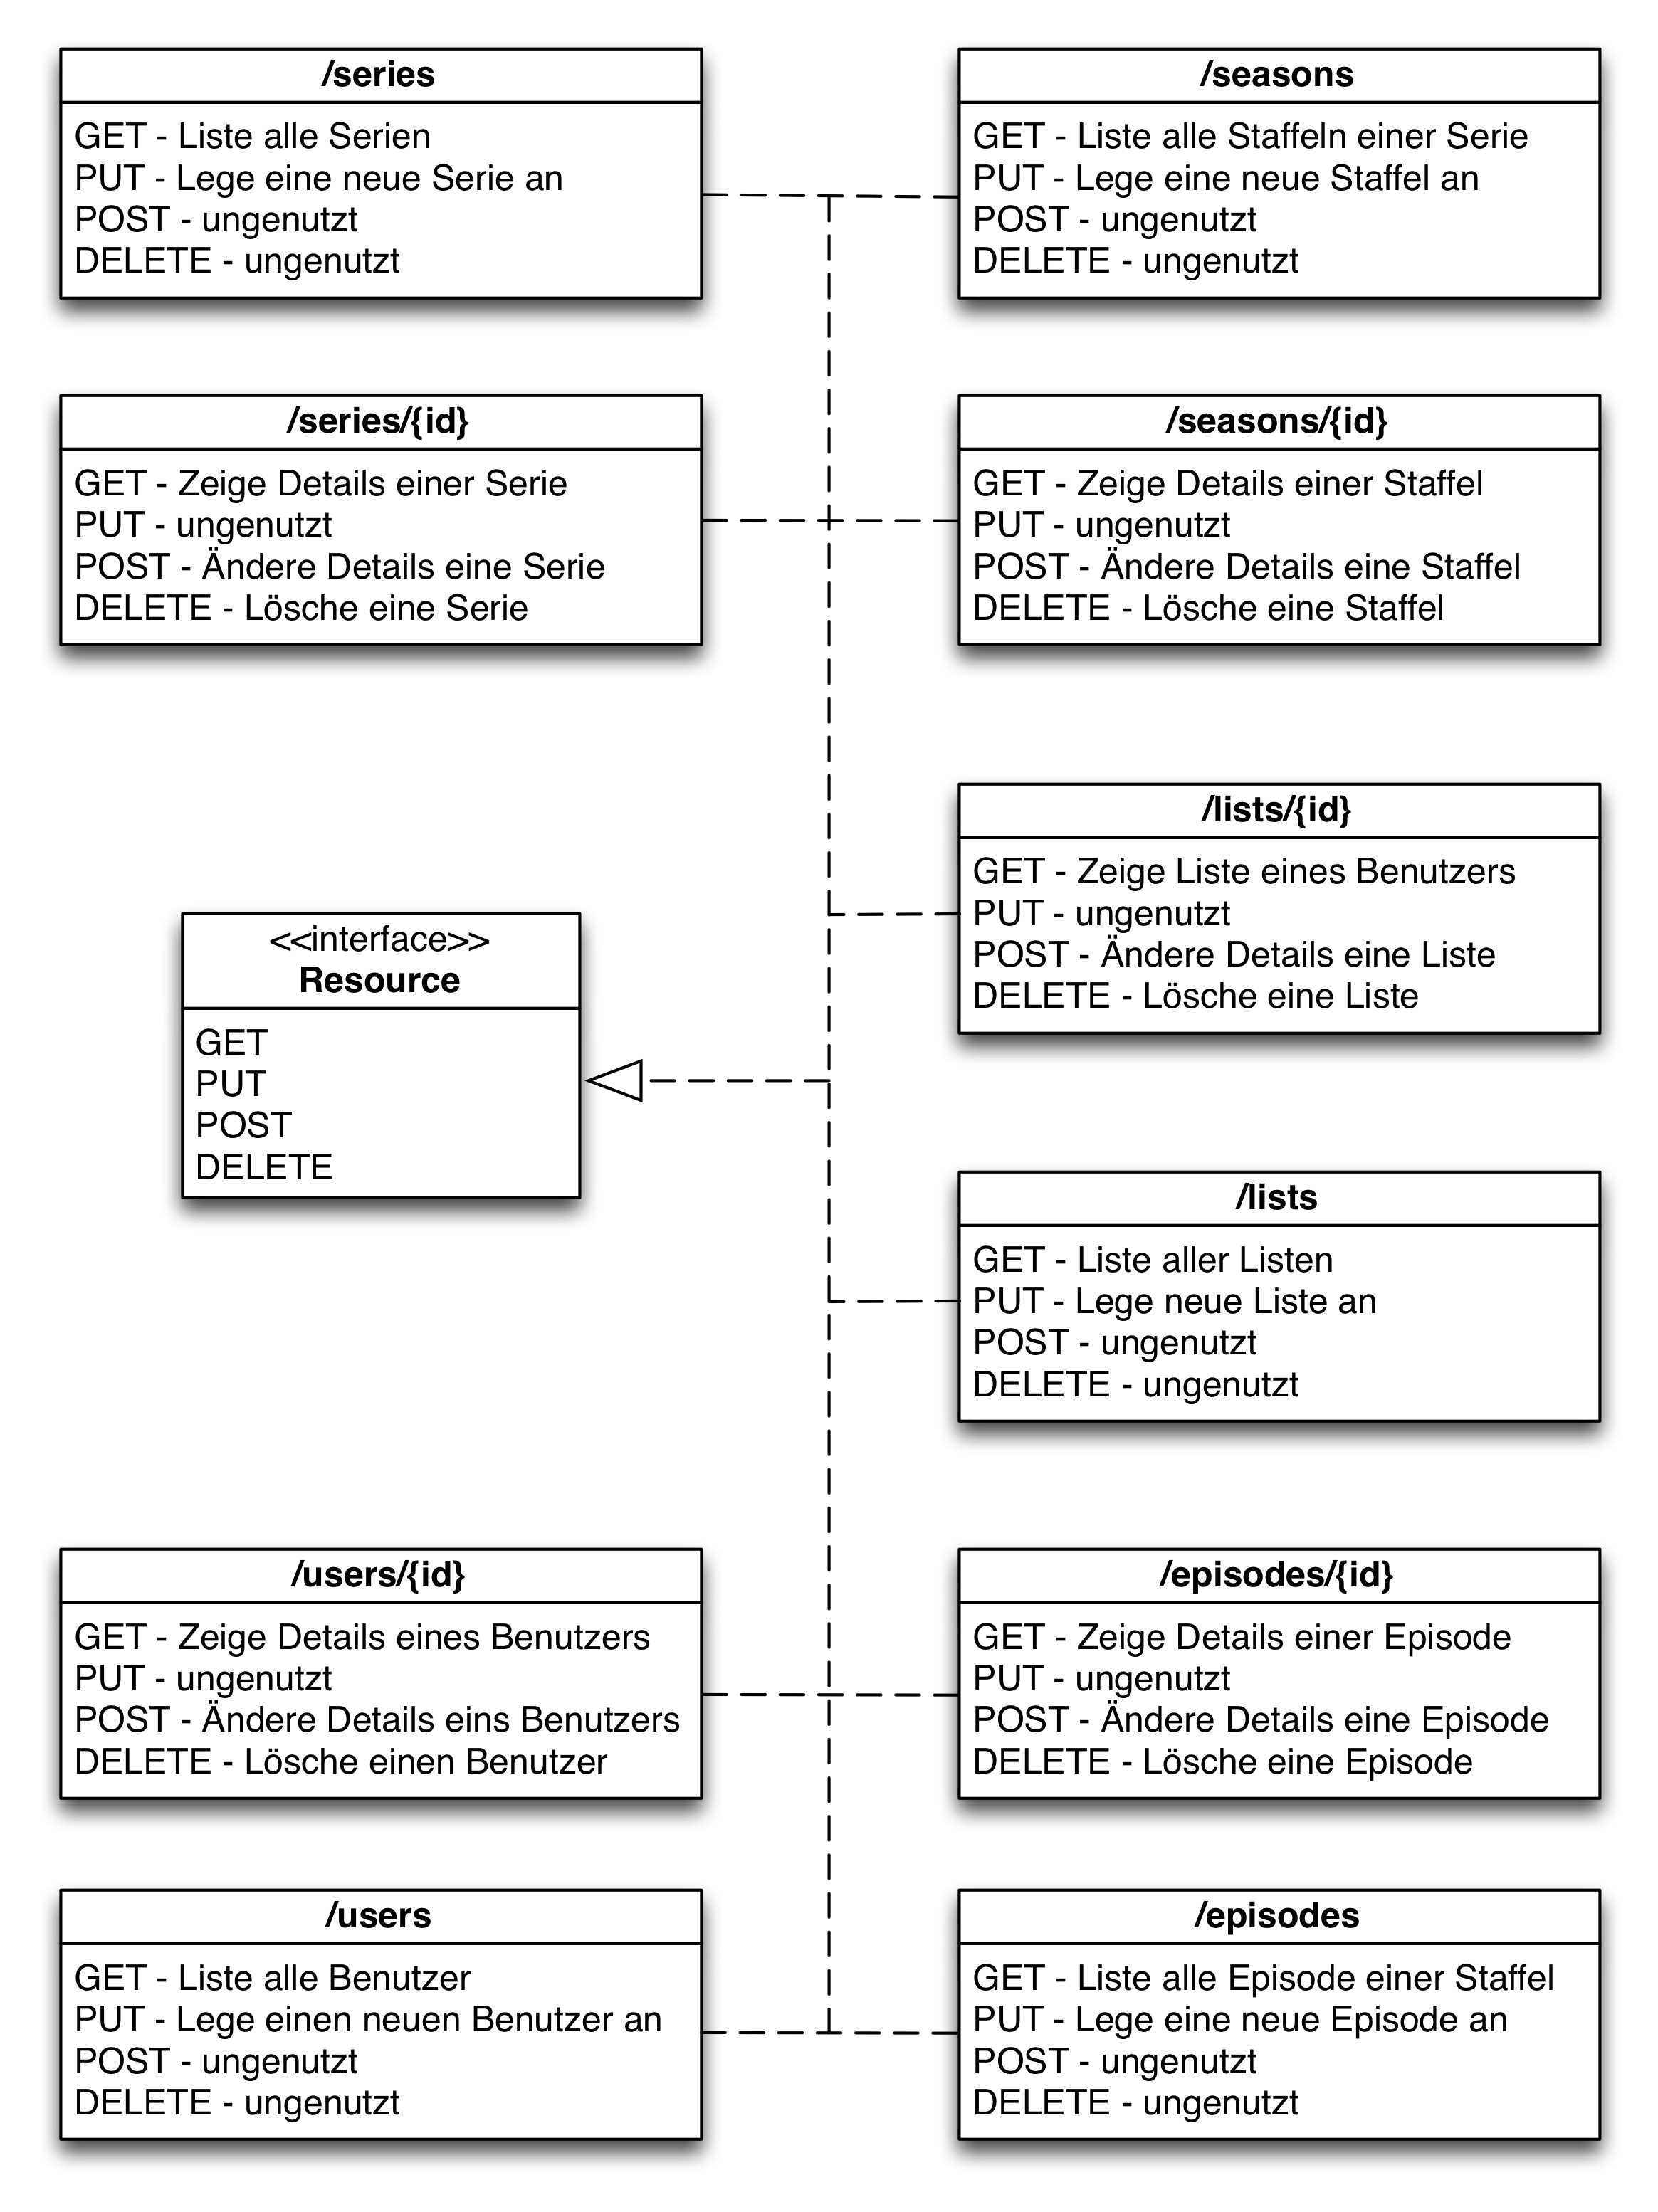
\includegraphics[width=.9\textwidth]{../images/bedeutunghttpmethoden.png}
\caption{Bedeutung der http Methoden}
\label{bedeutunghttpmethoden}
\end{figure}
